% citazioni, immagini

\chapter{Photo detectors}
After the scintillation phase in the crystal, visible photons are generated and coupled to a photodetector. At this stage the photodetector generates an eletric signal related to the photon rate, by generating free electrons in vacuum or electron-hole pairs in a semiconductor.

As they are used as fundamental components of the experimental apparatus the vacuum photodetector technology and the solid state technology will be presented.
Vacuum photodetectors are characterized by the production of free electrons in an external photocathode by photoelectric interaction. The produced electrons undergo acceleration in a focused electric field and are multiplied by secondary interaction before being transfered to the read out circuitry. Photo multiplier tubes (PMT) and micro channel plates (MCP) are prominent examples of vacuum technology.
  
In the case of solid state photo detectors, photons interact directly in the bulk material, where electron-hole pairs are produced. The pairs are then accelerated in the electric field and multiplied by ionization in the semiconductor itself. In the work presented here, Silicon photo multipliers (SiPM) are used as representative of this kind of detector.     

\section{Photo multiplier tubes}

Photo multiplier tubes are largely used vacuum photo detection devices and have been diffusively discussed in literature\cite{Knoll2000}. 
\begin{figure}[htbp]
\begin{center}
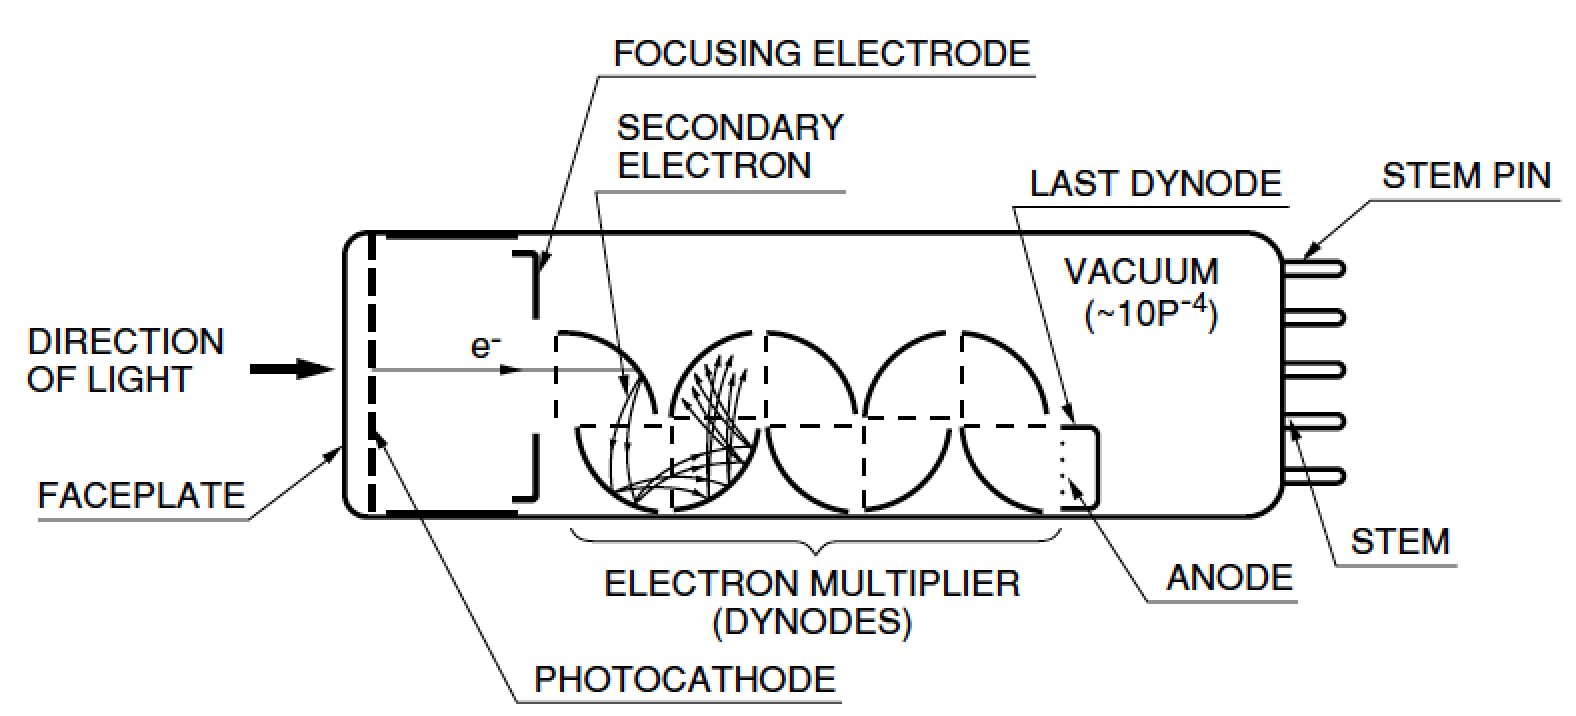
\includegraphics[width=12cm]{../Pictures/Chapter_3/PMT.png}
\end{center}
\caption[PMT schematics]{Schematics of a Photo-Multiplier Tube}
\label{fig:PMT_schematics}
\end{figure}
In figure \ref{fig:PMT_schematics} the main elements of a photo multiplier tube are sketched:
\begin{itemize}
\item a photocathode, which converts visible photons into an electron flux
\item an electron-optical input system which focuses and accelerates the electron flux
\item an electron multiplier consisting of a series of secondary emission electrodes (dynodes)
\item an anode, which collects the electron flux and supplies the output signal
\end{itemize}
Photoemission is due to a fraction of the incident visible photons that transfer enough energy to the electrons of the photo cathode to extract them.
Then the focusing system allows the freed electrons to reach the first dynode, i.e. the first multiplication stage. The electrons are accelerated and focused by eletric field between the dynodes and the required potential gradient is usually guaranteed by a voltage divider.

%foto divider

\subsection{Properties of PMT}
\begin{itemize}
\item \textbf{quantum efficiency}: photocathode are usually made of deposited photo emissive semiconductor. They can be semi transparent or opaque, depending on the place where the emissive material is deposited with respect to the input window.
The most used materials are silver-oxygen-caesium ($AgOCs$), antimonyum caesium ($SbCs$), and the bi-and trialkali compounds $SbKCs$, $SbRbCs$, and $SbNa_{2}KCs$. The most important parameter to be considered is the cathode radiant sensitivity, defined as the ratio of the cathode current $I_{p}$ to the incident flux $\Phi$
\begin{equation}
S_{k}(A/W)=\frac{I_{p}(A)}{\Phi _{e}(W)}
\end{equation}
The incoming photons have usually a certain spectral composition and the cathode is not uniformly sensitive in this range. With this respect the most used quantity is the quantum efficiency, that is the ratio of the number of photo electrons emitted, $n_{k}$, to the number of incident photons, $n_{i}$
\begin{equation}
QE = \frac{n_{k}}{n_{i}} = S_{k, \lambda} \frac{h\ni}{e}
\end{equation}
where $S_{k, \lambda}$ is the monochromatic sensitivity, defined as
\begin{equation}
S_{k, \lambda} = \lim_{d\lambda \to 0}\frac{dI_{p}}{d\Phi _{e}}
\end{equation}
%foto QE

\item \textbf{gain}: if the number of photo electrons that reach the first dynode is $n$, and the gain of the dynode is $g_{1}$, the number of secondary electrons is $n\cdot g_{1}$. If $g_{i}$ is the gain of the single dynodes, after $N$ stage the number of electrons collected at the anode are
\begin{equation}
n_{a} = n\prod_{i=1}^N g_i
\end{equation}
It is possible to define the gain of the photo multiplier as the ratio $I_{a}/I_{p}$ where $I_{a}$ is the anode current given by a photo current $I_{p}$. If we define a collection efficiency for each dynode, depending of geometrical parameters, $\eta _{i}$, then the gain $G$ is
\begin{equation}
G = \eta \prod_{i=1}^N \delta _{i} \eta _{i} = \eta \prod_{i=1}^N g_{i}
\end{equation}
\item \textbf{transit time spread}: transit time spread is the transit-time fluctuation of the signal when identical light pulses hit the same part of the ohiti cathode. The time resolution of a tube is then often quoted as the FWHM of the probability distribution of the fluctuations.
If the probability distribution of electrons arriving at the andode is assumed to be gaussian, then the response $R_{\delta}(t)$ to a delta-function light pulse is
\begin{equation}
R_{\delta}(t) = \frac{1}{\sigma _{R}\sqrt {2\pi}}exp\left( -\frac{(t-t_{tts})^2}{2\sigma _{R}^2}\right)
\end{equation}
where $t_{tts}$ is the mean transit time.
\end{itemize}

\section{Micro Channel Plate-PMT}
A micro channel plate is a two-dimensional array of glass capillaries mounted in parallel as shown in fig \ref{fig:MCP_schematics}.
\begin{figure}[htbp]
\begin{center}
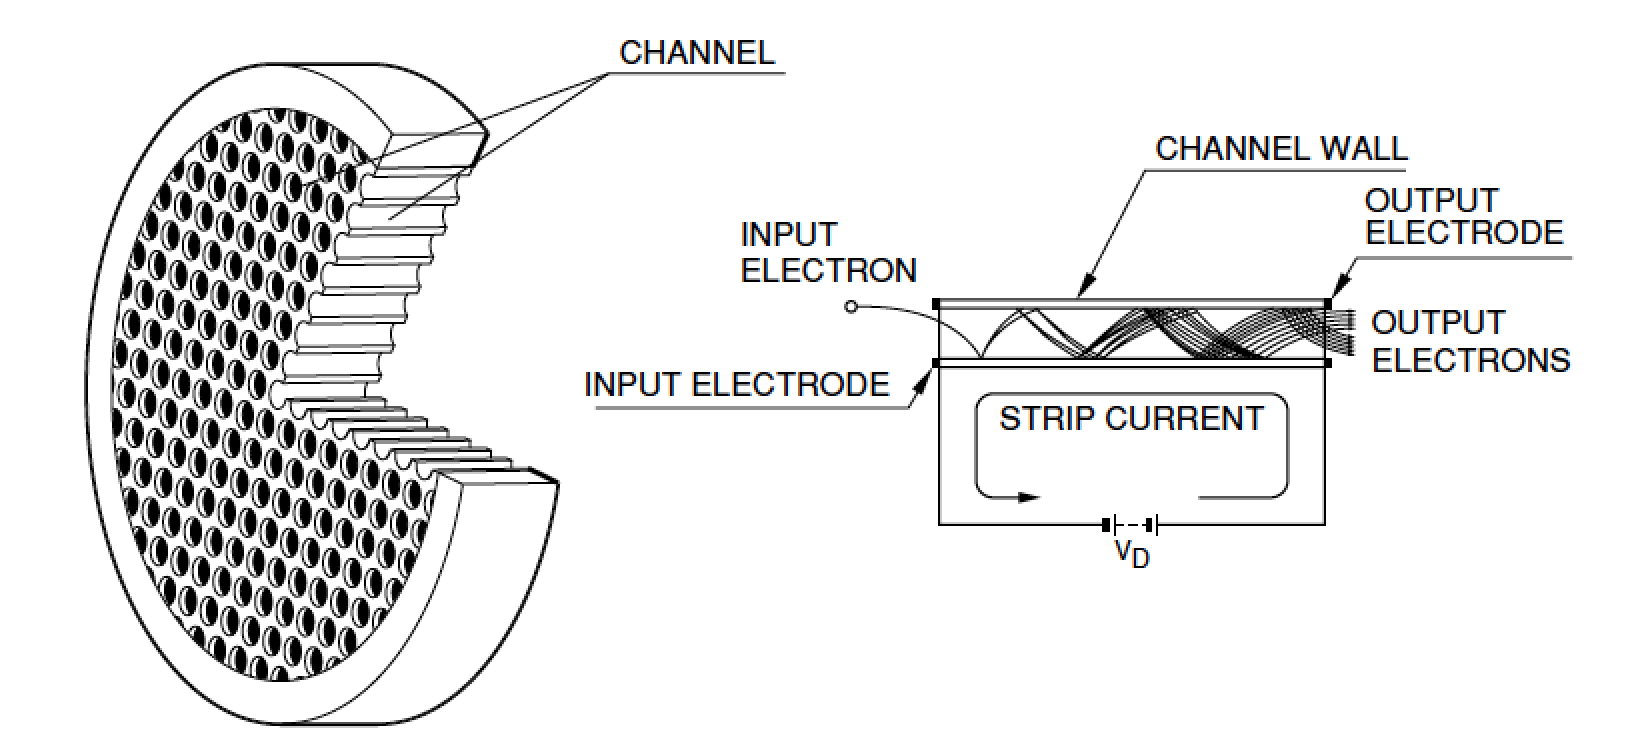
\includegraphics[width=12cm]{../Pictures/Chapter_3/MCP_plate.png}
\end{center}
\caption[MCP principle]{Work principle of a Micro Channel Plate}
\label{fig:MCP_schematics}
\end{figure}
The diameter of the channels lies in a range of 5 to 20 microns and their internal walls are treated so to hava a defined electrical resistance and secondary emissive properties.
At both ends of the plate high voltage is applied, so that a primary electron impinging on the wall of a channel produces a multiplication chain.
Since they resemble in function a structure of dynode, microchannel plates are usually used in combination with vacuum detector technology in an assembly known as MCP-PMT.
An MCP-PMT consists of an entry window, a photo cathode one or more micro channel plates and a collecting anode.
%MCP-PMT
To operate and MCP it is necessary to provide a certain voltage to the system. To this purpose standard voltage divider circuits are usually adopted, in order to guarantee mostly drifting spaces for electrons before and after the photocathode and multiplication in the MCP stack\cite{Hama2006}.
%divider  

  
\subsection{Properties of MCP}
\begin{figure}[htbp]
\begin{center}
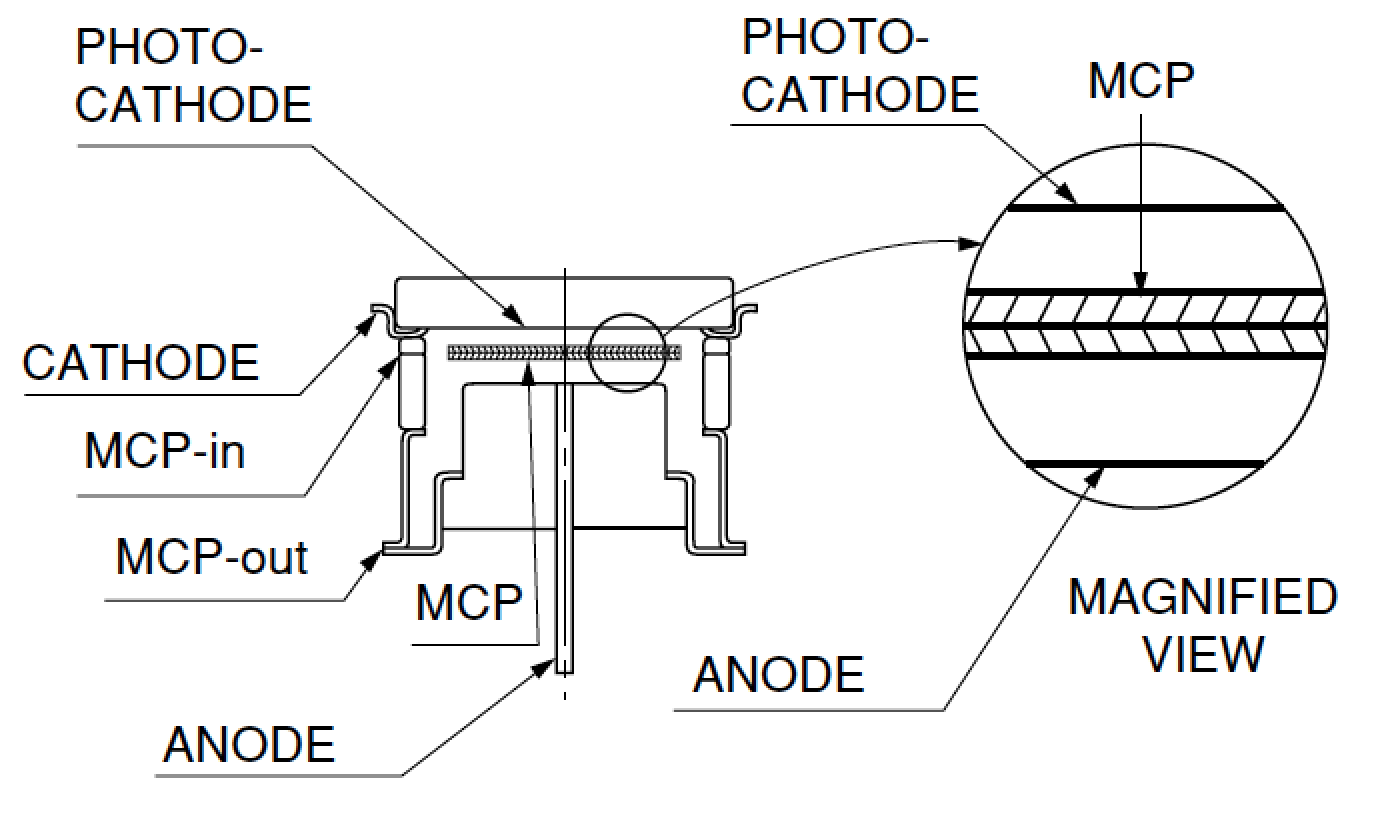
\includegraphics[width=12cm]{../Pictures/Chapter_3/MCP_struct}
\end{center}
\caption[MCP schematics]{Schematics of a MCP-PMT}
\label{fig:MCP_struct}
\end{figure}
\begin{itemize}
\item \textbf{quantum efficiency}: in terms of quantum efficiency they do not differ from standard PMTs, since they make use of the same technology in terms of photo cathodes.
\item gain
The gain of an MCP-PMT depends primarily on the number of plates stacked. Geometrically is determined by the length-to-diameter ratio af a channel $\alpha$, as
\begin{equation}
G = \exp{\left( \frac{\Delta \cdot L}{d} \right)} = \exp{\left( \Delta \cdot \alpha \right)}
\end{equation}
where $Delta$ is the gain factor and depends on the plate material, $L$ and $d$ are, respectivelly, the length and diameter of the micro tube.
%gain curve
\item \textbf{ion feedback, electron backscattering}: strongly correlated with the characteristics of gain are the problems of ion-feedback and electron backscattering. As the voltage, and thus the gain, increases, it is more and more likely for a photoelectron to be backscattered towards the photo cathode or for an ion to undergo the same process from the stack. Ions can be commonly stripped from residual gas in the drifting area or from interaction in the plate.
This leads to the production of secondary pulses, that contribute in the worsen of the time response of the device.
Connected to this is also the issue of ageing, since ion bombardment damages the photocathode and it is more and more likely as the vacuum in the device degrades with time.
Partial solution to this problem has been found by depositing an Aluminum protection layer on the plate and by modifying the inclination of the micro tubes in the so called Chevron geometry\cite{Vavra2004}.
%immagine su ion feedback

\item \textbf{time characteristics}: the rise and fall time of a MCP-PMT are ultra-short, due to the multiplication characteristics of the device. This translated into typical signal contained in a few nanoseconds, or even less. For timing application though the most important parameter to consider is the transit time spread (TTS). The TTS is the spread in the arrival time of a bunch of photon produced by a converted electron in the photocathode. The time response of MCP-PMTs will be analyzed further in the next chapters.

%typical IRF
\end{itemize}

\section{Silicon photo multipliers}
Recently solid state photo detectors have become competitive with vacuum devices, and for some applications they represent the ideal solution. Their advantage lies in the high photon detection efficiency, their low sensitivity to high magnetic fields, their compactness and cost efficiency\cite{Dolgoshein2003}.
In particular the insensitivity to high magnetic fields, given by the feature that no electrons are travelling in the vacuum between dynode and dynode, makes the solid photo detector the first choice for PET-MRI scanners or high energy experiments. With respect to the MCP-PMT, also characterized by high operability in magnetic fields, silicon devices still mantain a high photon detection efficiency, that is the conversion efficiency of incoming photons in to electron hole pairs determining in principe a better energy and time resolution.
\begin{figure}[htbp]
\begin{center}
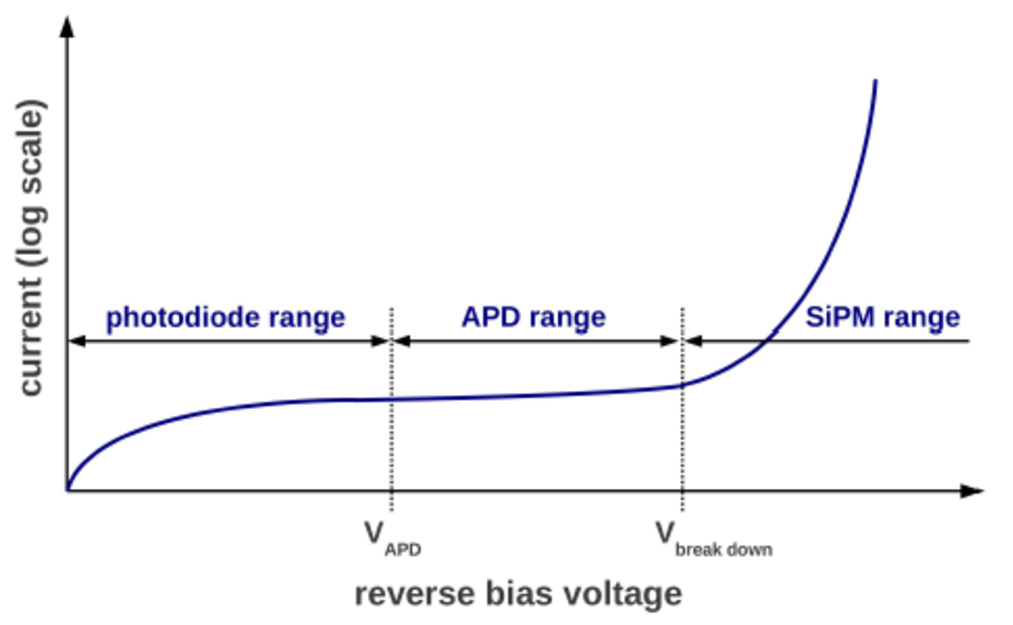
\includegraphics[width=12cm]{../Pictures/Chapter_3/avalanche.pdf}
\end{center}
\caption[I-V plot Silicon detectors]{Voltage current plot for Silicon devices. SiPMs work in Geiger mode.}
\label{fig:avalanche}
\end{figure}

Solid state photo detectors are usually p-n junctions biased reversely and depending on the value of the bias voltage different operational parameters adapt to fundamentally three modes.
As seen in figure \ref{fig:avalanche} the voltage can applied can be low, as in photo diodes, leading to low currents proportional to the incoming flux. Moving towards the proportionality region the freed electrons are able to ionize further, thus determining a net gain of the device. Avalanche photodiodes (APDs) are a common device operated in this region.
Finally a third region, characterized by non-proportionality is the precipous operating segment of Geiger mode APD (G-APD). In the Geiger mode region both electrons and holes are able to futher ionize the bulk, and the device is sensible to single photo electrons. The created avalanche must be quenched either externally by a series of quenching resistors or actively.
Many G-APD cells connected in parallel are the basic structure of silicon photo-multipliers (SiPM) or multi pixel photon counters (MPPC).

\begin{figure}
\centering
\begin{subfigure}
  {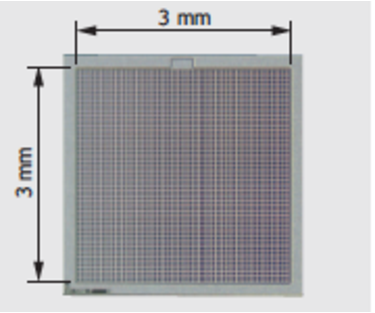
\includegraphics[width=6cm]{Pictures/Chapter_3/mppc_photo.pdf}}
\end{subfigure}
\begin{subfigure}
  {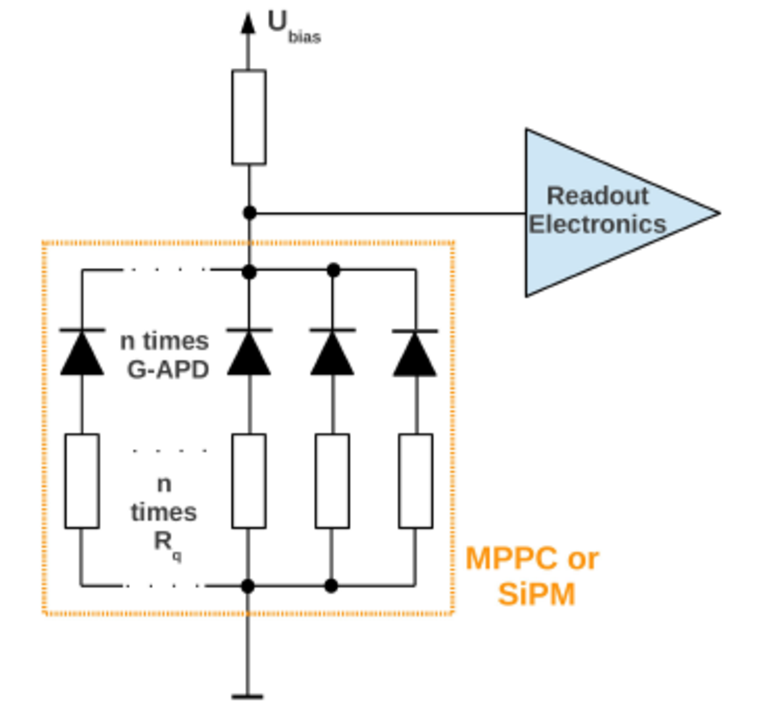
\includegraphics[width=6cm]{Pictures/Chapter_3/mppc_schema.pdf}}
\end{subfigure}
\caption[Example of SiPM]{Example of Hamamatsu MPPC (left) and basic strucutre of a SiPM (right)}
\label{fig:mppc}
\end{figure}

\subsection{Analog SiPM}
The structure of an analog SiPM is composed by series of Geiger mode cells in parallel, and the self sustained avalanche is usually quenched by external resistors or active quenching circuitry. The basic schema of a standard SiPM with quenching resistors is shown in figure \ref{fig:mppc}.

The structure of a G-APD optimized for detection of blue light is shown in figure \ref{fig:uvir}.
On top of the low resistivity bulk layer an epitaxial layer with a high dopant concetration region is located.
The implantation of opposite charge consitutes the p-n junction with a very thin layer extremely doped to assure electric field uniformity.
The cell and the quenching resistor are connected on the top surface.
Finally a passivation layer (SiO2) protects the device. Due to its low index of refraction ($1.55$ in the blue) with respect to the one of Silicon ($3.5$) Fresnel losses can occurr, usually compensated by the presence of anti-reflection coatings.

\begin{figure}
\centering
\begin{subfigure}
  {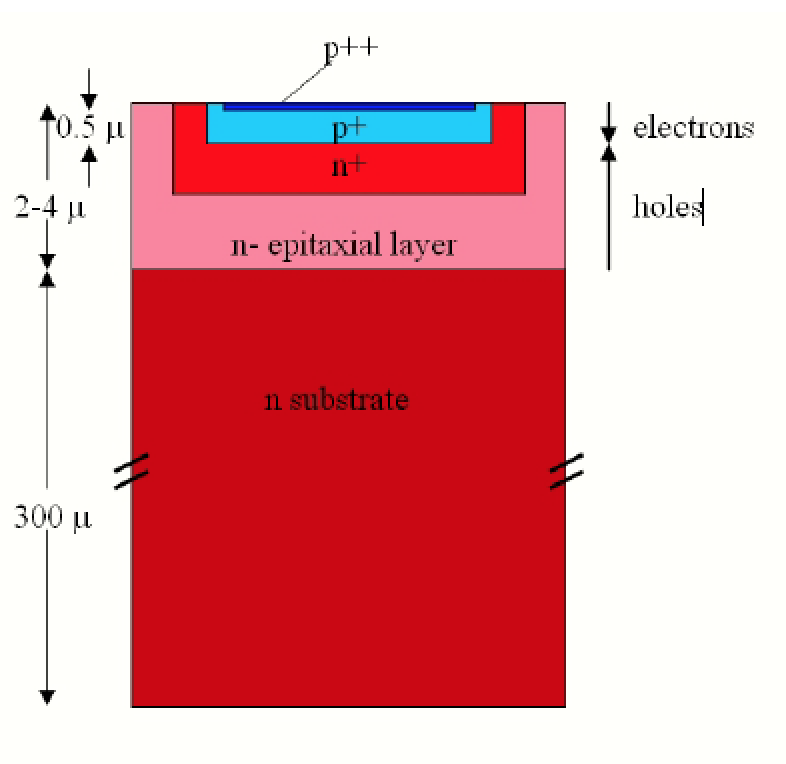
\includegraphics[width=6cm]{Pictures/Chapter_3/IR_mppc}}
\end{subfigure}
\begin{subfigure}
  {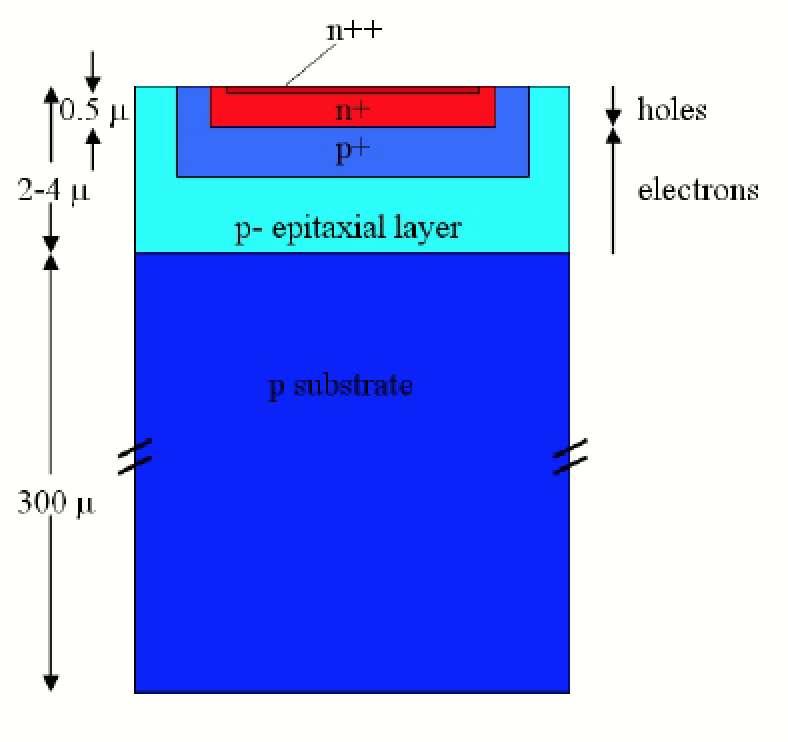
\includegraphics[width=6cm]{Pictures/Chapter_3/UV_mppc}}
\end{subfigure}
\caption[SiPM layer structure]{Layered structure of a IR (left) and UV (right) SiPM}
\label{fig:uvir}
\end{figure}

\subsection{Properties of SiPM}
\begin{itemize}
\item \textbf{photon detection efficiency}: the photon detection efficiency can be defined as
\begin{equation}
PDE = QE \cdot \epsilon \cdot P_{avalanche}
\end{equation}
where $QE$ is the quantum efficiency, $\epsilon$ is the geometric fill factor and $P_{avalanche}$ is the probability of triggering an avalanche.
The $QE$ has already been introduced for ordinary photo cathodes and it is comprehensive of Fresnel losses.
The fill factor $\epsilon$ is defined as the ratio of the sensitive area to the total area of the detector.
Finally the $P_{avalanche}$ is the probability of an electron or hole to cause an avalanche and it depends on the bias overvoltage.
% tipical value

\item \textbf{gain}: the gain of an analog SiPM can be written as
\begin{equation}
G = \frac{C\cdot U_{ov}}{q}
\end{equation}
where $C$ is the cell capacitance, $U_{ov}$ is the bias overvoltage and $q$ is the charge $q = 1.602 \cdot 10^{-19} C$.
This value is tipically between $10^{5}$ and $10^{7}$.

\item \textbf{spurious events} a dark count is the random production of charge carriers in the depleted region which leads to a regular signal. This type of unwanted event is tipically uncorrelated, provided the the darc count rate (DCR) is low enough. It strongly depends of temperature, and typical values range between $100kHz$ to few $MHz$ at $25C$.
Optical crosstalk on the other hand is determined by the trigger of an avalanche by an optical photon produced in a neighbouring cell. Indeed optical photons produced in avalanches can travel to other cells, causing correlated spurious pulses. These pulses can occur even after a delay of several microseconds, due to the secondary photons generating electron hole pairs.
Moreover charge carriers can be trapped in the bulk and released tens to hundreds of nanoseconds later determining afterpulsing.

\item \textbf{saturation}: if SiPMs are exposed to high photon fluxes, saturation effects may occurr. The detector is intrinsically limited by the number of cells: if the number of photons is small compared to the number of cells provided PDE correction, the SiPM signal is proportional to the light signal. In the opposite case, the signal is saturated.
\end{itemize}

\subsection{The NINO chip}
Signal generated by SiPMs are in the range of  
Thus we make use of low noise electronics to read out the detector. In the study presented the ultrafast front-end preamplifier-discriminator chip called NINO, developed at CERN\cite{Anghinolfi2004}. Originally designed for the time-of-flight subdetector of the ALICE experiment, it matches the main requirements of a SiPM readout, that is speed, low noise, minimum slew rate, low input impedance.
The chip has eight channels, designed for differential readout. Each channel is is characterized by an amplifier with 1-ns peaking time, a discriminator with a minimum detection threshold of 10 fC and an output stage.

\begin{figure}
\centering
\begin{subfigure}
  {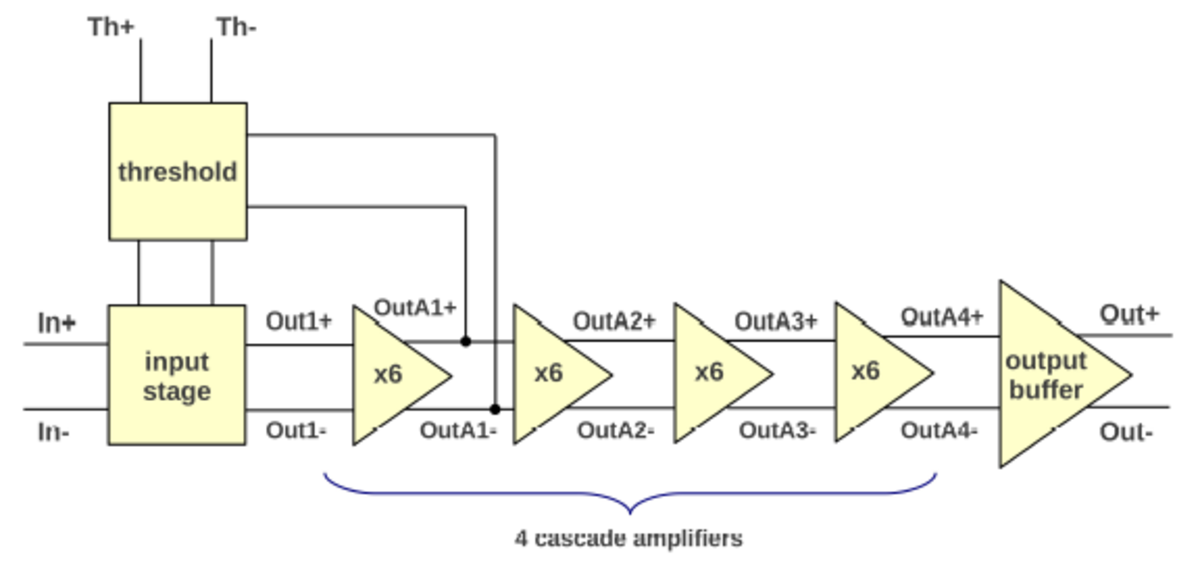
\includegraphics[width=6cm]{Pictures/Chapter_3/NINO_scheme.pdf}}
\end{subfigure}
\begin{subfigure}
  {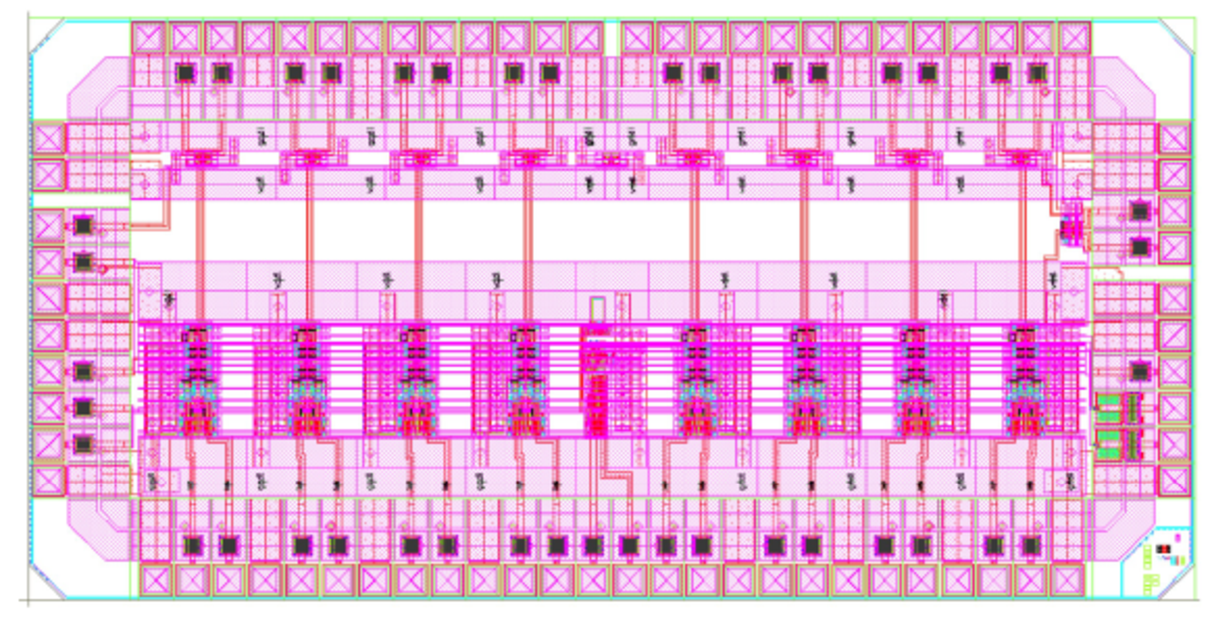
\includegraphics[width=6cm]{Pictures/Chapter_3/NINO.pdf}}
\end{subfigure}
\caption[NINO chip]{Structure of the cascade amplifier (left) and scheme (right) of the NINO chip}
\label{fig:nino}
\end{figure}

The input stage is a current-to-voltage converter and the subsequent signal amplification is performed with four identical cascade amplifiers that operate as a discriminator as well.
The threshold is set by a voltage difference applied on two symmetrical inputs.
The NINO chip makes use of the time-over-threshold technique: a squared output pulse is produced when the leading edge is above the set threshold, encoding the timing information. The width of this signal, on the other hand, is a function of the charge collected, thus encoding the energy information. 

\begin{figure}[htbp]
\begin{center}
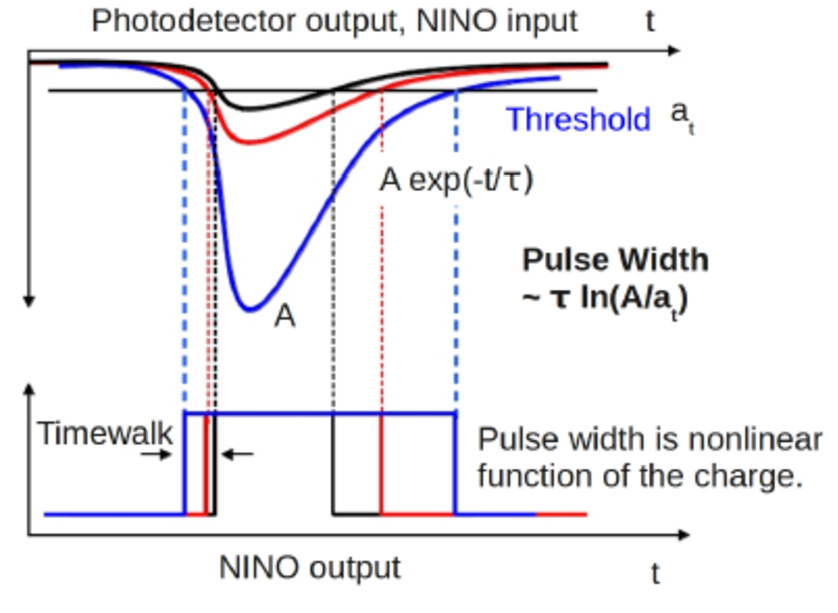
\includegraphics[width=9cm]{../Pictures/Chapter_3/TOT.pdf}
\end{center}
\caption[Time-over-threshold]{Principle of operation of a time-over-treshold discriminator}
\label{fig:tot}
\end{figure}

